\documentclass[border=10pt]{standalone}
\usepackage[svgnames]{xcolor}
\usepackage{amsmath}
\usepackage{pgfplots}
\pgfplotsset{compat=newest}
\usepackage[sfdefault]{FiraSans}
\usepackage{FiraMono}
\renewcommand*\familydefault{\sfdefault}
\begin{document}
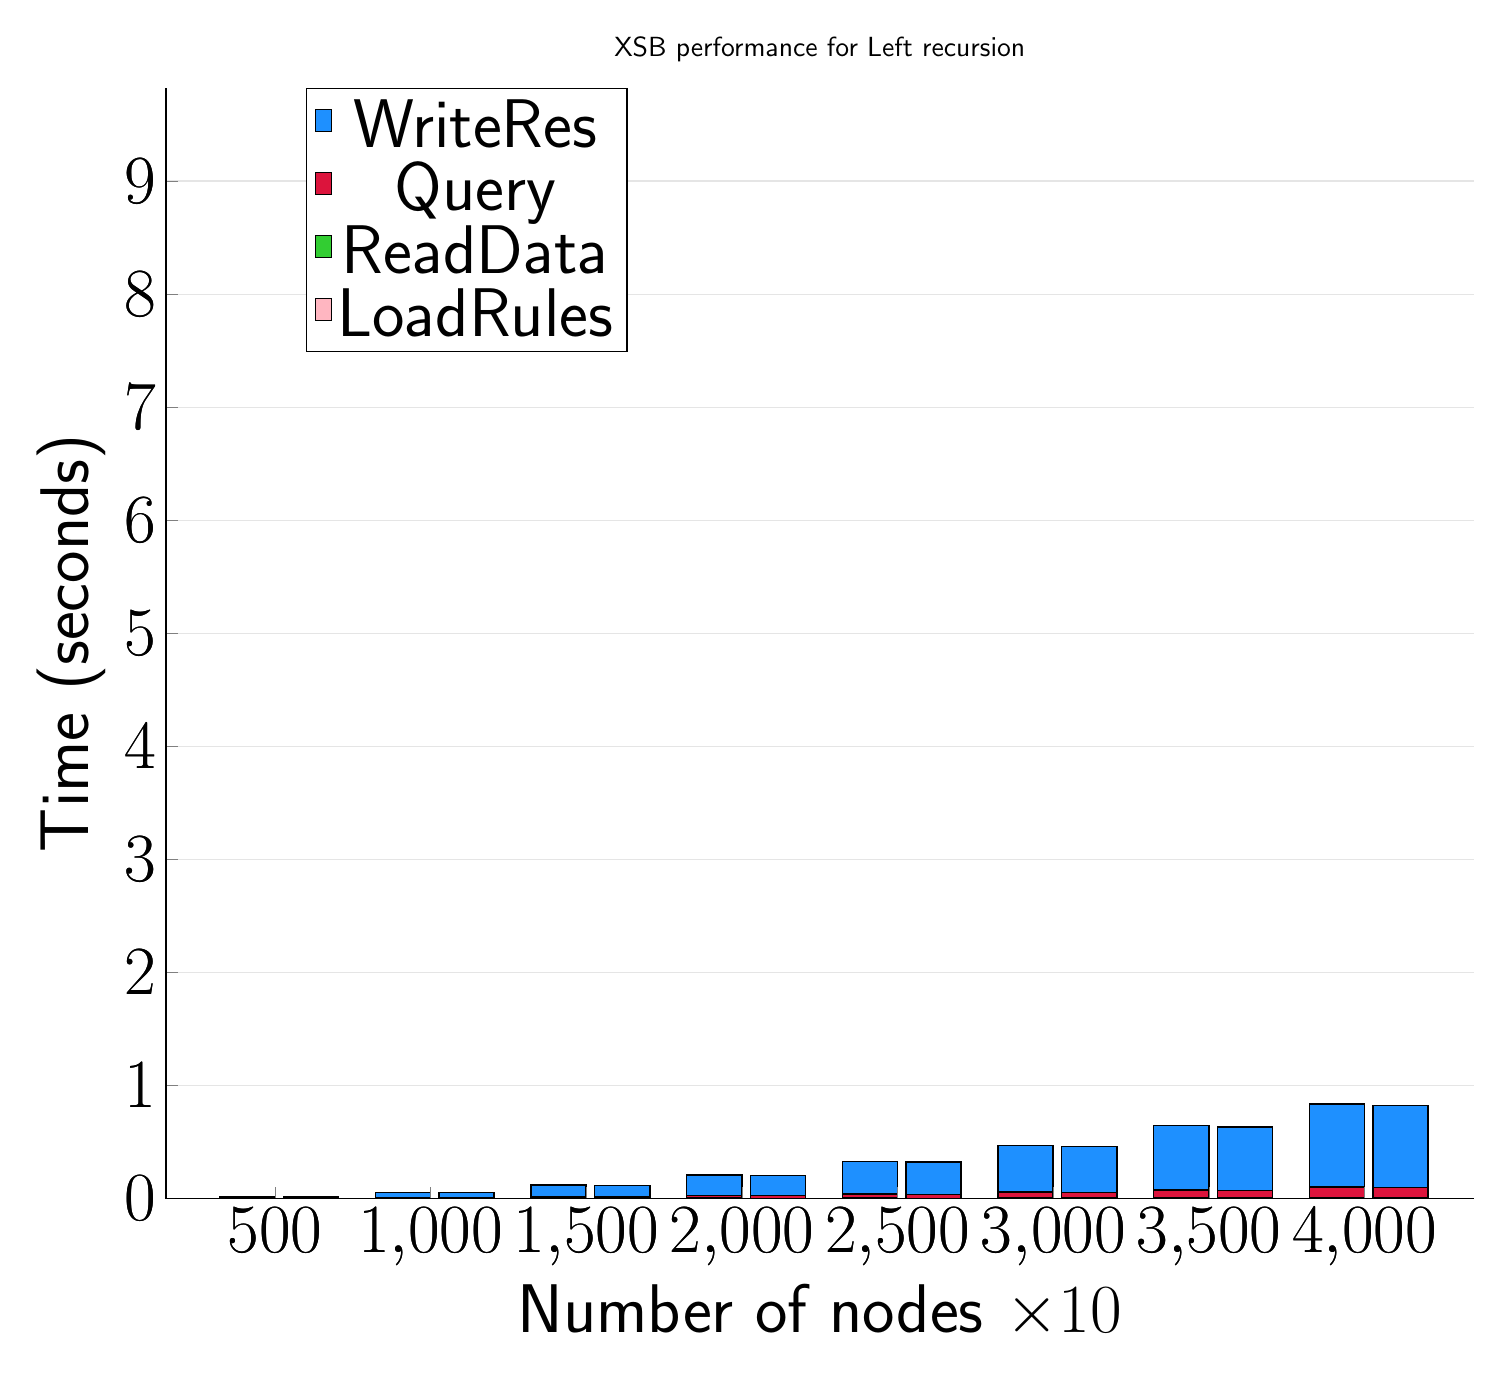
\begin{tikzpicture}
	\begin{axis}[
			ybar stacked,
			title={XSB performance for Left recursion},
			bar shift=-10pt,
			width=1.5\textwidth,
			bar width=0.7cm,
			ymajorgrids, tick align=inside,
			major grid style={draw=gray!20},
			xtick=data,
			ymin=0, ymax=9.824258804321289,
			axis x line*=bottom,
			axis y line*=left,
			enlarge x limits=0.1,
			legend style={
					at={(0.23, 1)},
					anchor=north,
					legend columns=1,
					font=\Huge,
				},
			ylabel={Time (seconds)},
			xlabel={Number of nodes $\times 10$},
			label style={font=\Huge},
			tick label style={font=\Huge},
		]
		\addlegendimage{fill=DodgerBlue, draw=black, line width=0.2pt}
		\addlegendentry{WriteRes}
		\addlegendimage{fill=Crimson, draw=black, line width=0.2pt}
		\addlegendentry{Query}
		\addlegendimage{fill=LimeGreen, draw=black, line width=0.2pt}
		\addlegendentry{ReadData}
		\addlegendimage{fill=LightPink, draw=black, line width=0.2pt}
		\addlegendentry{LoadRules}
		\addplot +[fill=LightPink, draw=black, line width=0.5pt] coordinates {
				(500, 0.0010848522186279312)
				(1000, 0.0010660648345947271)
				(1500, 0.0010406494140624992)
				(2000, 0.0010607242584228529)
				(2500, 0.0010730266571044931)
				(3000, 0.001087164878845214)
				(3500, 0.0011159658432006833)
				(4000, 0.001102900505065917)
			};
		\addplot +[fill=LimeGreen, draw=black, line width=0.5pt] coordinates {
				(500, 0.000810694694519043)
				(1000, 0.001274728775024415)
				(1500, 0.001759910583496094)
				(2000, 0.0022651910781860346)
				(2500, 0.002794480323791506)
				(3000, 0.0033098936080932623)
				(3500, 0.00380070209503174)
				(4000, 0.004274129867553709)
			};
		\addplot +[fill=Crimson, draw=black, line width=0.5pt] coordinates {
				(500, 0.001426911354064942)
				(1000, 0.005548715591430663)
				(1500, 0.01242225170135498)
				(2000, 0.023247051239013668)
				(2500, 0.03548865318298337)
				(3000, 0.052513527870178225)
				(3500, 0.0715418815612793)
				(4000, 0.09653756618499755)
			};
		\addplot +[fill=DodgerBlue, draw=black, line width=0.5pt] coordinates {
				(500, 0.01192593574523926)
				(1000, 0.04703819751739502)
				(1500, 0.10467071533203132)
				(2000, 0.18328385353088364)
				(2500, 0.2902926206588745)
				(3000, 0.41509058475494404)
				(3500, 0.5682461500167845)
				(4000, 0.7361536741256716)
			};
	\end{axis}
	\begin{axis}[
			ybar stacked,
			bar shift=13pt,
			width=1.5\textwidth,
			bar width=0.7cm,
			ymajorgrids, tick align=inside,
			major grid style={draw=none},
			xtick=data,
			ymin=0, ymax=9.824258804321289,
			axis x line*=none,
			axis y line*=none,
			enlarge x limits=0.1,
			label style={font=\Huge},
			tick label style={font=\Huge},
		]
		\addplot +[fill=LightPink, draw=black, line width=0.5pt] coordinates {
				(500, 0.0006144000000000004)
				(1000, 0.0006170000000000001)
				(1500, 0.0006036000000000001)
				(2000, 0.0006014000000000002)
				(2500, 0.0006100000000000003)
				(3000, 0.0006083000000000001)
				(3500, 0.0006330999999999999)
				(4000, 0.0006348999999999995)
			};
		\addplot +[fill=LimeGreen, draw=black, line width=0.5pt] coordinates {
				(500, 0.0005751999999999997)
				(1000, 0.001001399999999999)
				(1500, 0.0014525)
				(2000, 0.0019239000000000003)
				(2500, 0.0023976)
				(3000, 0.0028595)
				(3500, 0.0032928)
				(4000, 0.0037789000000000004)
			};
		\addplot +[fill=Crimson, draw=black, line width=0.5pt] coordinates {
				(500, 0.0013463999999999998)
				(1000, 0.005301599999999999)
				(1500, 0.0119086)
				(2000, 0.0221653)
				(2500, 0.0338746)
				(3000, 0.050072799999999994)
				(3500, 0.0680577)
				(4000, 0.0915405)
			};
		\addplot +[fill=DodgerBlue, draw=black, line width=0.5pt] coordinates {
				(500, 0.011429)
				(1000, 0.046037499999999995)
				(1500, 0.10270350000000002)
				(2000, 0.18078100000000003)
				(2500, 0.2857507)
				(3000, 0.4086659)
				(3500, 0.5595814000000001)
				(4000, 0.7277069)
			};
	\end{axis}
\end{tikzpicture}

\end{document}
